% =========================================================================
% SECTION 5.6: SIMULATION OF TWO QUADRANT CHOPPER (ACTUAL RATINGS)
% =========================================================================
\section{Simulation of Two Quadrant Chopper (Actual Ratings)}

\subsection{Bidirectional CC-CV Supervisory Energy Management System}

\subsubsection{Introduction}
The inherently intermittent and stochastic nature of solar photovoltaic (PV) generation poses significant challenges to maintaining a stable and reliable charging profile. To mitigate these power fluctuations and decouple the EV charging load from weather-dependent variables, the inclusion of a localized Energy Storage System (ESS) is essential.

To interface this ESS with the central DC link of the charging station, a power electronic topology capable of bidirectional energy transfer is mandatory. Traditional one-quadrant converters are insufficient, as they only permit unidirectional power flow. Therefore, this project implements a Two-Quadrant (2Q) DC-DC Chopper (configured as a synchronous bidirectional Buck-Boost converter) to serve as the core power conditioning interface for the ESS.

\subsubsection{Simulation Model}
\renewcommand{\thefigure}{5.\arabic{figure}}

\begin{figure}[H]
    \centering
    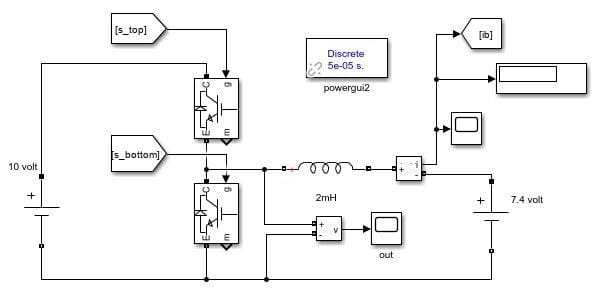
\includegraphics[width=0.8\textwidth]{Figures/2qcc.jpeg} 
    \caption{Two Quadrant chopper simulation model.}
    \label{fig:two_quad_simulation_model}
\end{figure}

\begin{figure}[H]
    \centering
    % --- FIRST SUBFIGURE ---
    \begin{subfigure}[b]{0.45\textwidth}
        \centering
        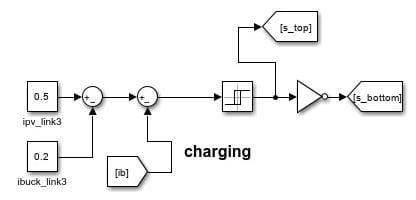
\includegraphics[width=\linewidth]{Figures/charging.jpg}
        \caption{Charging CC control.}
        \label{fig:charging_cc_sub}
    \end{subfigure}
    \hfill 
    % --- SECOND SUBFIGURE ---
    \begin{subfigure}[b]{0.45\textwidth}
        \centering
        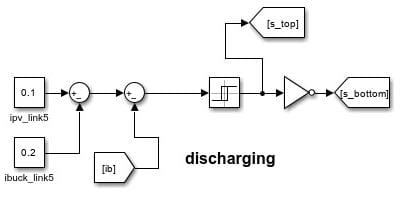
\includegraphics[width=\linewidth]{Figures/dischcc.jpg}
        \caption{Discharging CC control.}
        \label{fig:discharging_cc_sub}
    \end{subfigure}
    \caption{2Q Chopper constant current (CC) block configurations.}
    \label{fig:main_combined_cc_control}
\end{figure}

The complete architecture modeled within the MATLAB/Simulink environment is illustrated in Figure 5.1. The circuit consists of a high-voltage DC link representing the microgrid bus $V_{dclink} = 10\text{ V}$, a half-bridge IGBT/Diode switching leg, a power filtering inductor $L = 2\text{ mH}$, and a low-voltage battery storage system $V_{b} = 7.4\text{ V}$.

\subsubsection{Principle of Operation}
In traditional systems, current regulation is managed by a linear Proportional-Integral (PI) loop driving a carrier-based Pulse Width Modulation (PWM) modulator. While effective at a fixed operating point, linear control strategies often struggle when paired with highly non-linear loads such as chemical batteries, demanding complex tuning, anti-windup compensation circuitry, and undesirable trade-offs between dynamic response and steady-state stability.

To overcome these structural boundaries, this model deploys a non-linear Hysteresis Current Control (HCC) strategy. HCC is a direct, bang-bang control technique that monitors the instantaneous current error and switches the power semiconductors directly whenever the error crosses a pre-calculated tolerance band. This eliminates the intermediate PWM modulator entirely, resulting in a system with an inherently high dynamic bandwidth, unconditional stability, and an instantaneous response to transient source or load perturbations.

The control system evaluates the tracking error $e(t)$ in real time by subtracting the instantaneous feedback battery current $I_{b}$ from the computed reference target $I_{ref}$:
\begin{equation}
    e(t) = I_{ref} - I_{b}
\end{equation}

The logic applies a defined hysteresis band ($h$) via a relay block to determine the gating states:
\begin{align}
    \text{If } e(t) > +h &\implies S_{top} = 1,\; S_{bottom} = 0 \quad (\text{Current Increases}) \\
    \text{If } e(t) < -h &\implies S_{top} = 0,\; S_{bottom} = 1 \quad (\text{Current Decreases})
\end{align}

This control compares the reference current to the inductor current and uses a relay to switch the IGBTs instantly. This ensures a rapid response by keeping the $2\text{ mH}$ inductor current stable and bounded within its strict ripple thresholds.

Furthermore, the control architecture implemented in this simulation focuses exclusively on Constant Current (CC) regulation, while Constant Voltage (CV) control was intentionally omitted from the design scope. Because the primary objective of this 2Q Chopper simulation is to validate immediate, millisecond-level bidirectional power balancing during stochastic PV irradiance drops, implementing a slow, long-term CV loop was technically unnecessary. During bulk energy transfer and transient microgrid stabilization, the ESS battery pack operates strictly within its safe nominal State of Charge (SoC) boundaries, where the CC phase is dominant. This strategic design choice optimizes simulation execution speed and avoids redundant computational overhead while fully demonstrating the high-frequency dynamic capabilities of the bidirectional converter.

The simulation model shown before is a closed loop model working as a buck or boost converter depending on the following case scenarios.

\subsubsection{Modes and Quadrant Analysis}

\paragraph{Quadrant I: Excess Generation Phase (ESS Charging / Buck Mode)}
When environmental conditions are optimal, the power produced by the PV panels often exceeds the instantaneous demand required to charge the EV battery. To prevent overvoltage conditions on the shared DC link and maximize renewable energy capture, this surplus power must be actively redirected.

During this phase, the 2Q Chopper operates in Buck Mode. Current flows directly from the high-voltage DC link into the ESS, allowing the storage unit to function as a controllable load that safely absorbs the excess energy. The active control block diagram for this operational state is illustrated in Figure 5.2a.

\paragraph{Quadrant II: Generation Deficit Phase (ESS Discharging / Boost Mode)}
Conversely, during periods of reduced solar irradiance---such as cloud cover, shading, or late afternoon hours---the power production from the PV panels drops below the threshold required to sustain the EV battery's targeted charging rate.

To compensate for this sudden power drop, the 2Q Chopper seamlessly transitions to Boost Mode. The ESS shifts from a power sink to a primary source, forcing current to flow in the reverse direction---out of the ESS and up to the DC link---to complement the falling PV power and ensure an uninterrupted, stable charge for the electric vehicle. The control block configuration for this state is shown in Figure 5.2b.

\subsubsection{Design Parameters and Analytical Dimensioning}

\paragraph{System Specifications}
The core electrical parameter constraints of the developed simulation are summarized in Table 5.1.

\renewcommand{\thetable}{5.\arabic{table}}
\begin{table}[H]
    \centering
    \noindent
    \centerline{%
    \newcolumntype{C}{>{\centering\arraybackslash}X}
    \begin{tabularx}{\textwidth}{c l C}
        \toprule
        \textbf{Symbol} & \textbf{Parameter} & \textbf{Design Value} \\
        \midrule
        $V_{dclink}$ & DC link voltage & $10\text{ V}$ \\
        $V_{b}$      & ESS battery voltage & $7.4\text{ V}$ \\
        $I_{pvlink}$ & Source input current & Solar dependent ($0.5\text{ A}$ -- $0.1\text{ A}$) \\
        $I_{bucklink}$ & EV charging current & $0.2\text{ A}$ \\
        $I_{ref}$    & Reference current & $I_{pvlink} - I_{bucklink}$ \\
        $L$          & Inductance & $2\text{ mH}$ \\
        $H$          & Hysteresis band & $\pm 0.01$ \\
        \bottomrule 
    \end{tabularx}%
    }
    \caption{Two Quadrant Chopper Simulation Specifications.}
    \label{tab:chopper_specs}
\end{table}
\newpage
\paragraph{Inductor Ripple Analysis}
For a hysteresis-controlled converter, the maximum switching frequency $f_{swmax}$ and the inductor ripple current $\Delta i_{L}$ are coupled parameters. To guarantee that the ripple remains strictly within the designated control limits under all operating configurations, the inductor value must be cross-checked using both topological states.

\vspace{1.5ex}
\noindent\textit{Case 1: Buck Mode Sizing Formulation}\\
During the turn-on period of the upper switch $S_{top}$, the voltage across the inductor is $V_{dclink} - V_{b}$. The ripple current can be expressed analytically as:
\begin{equation}
    \Delta I_{buck} = \frac{(V_{dclink} - V_{b}) \cdot V_{b}}{L \cdot f_{sw} \cdot V_{dclink}}
\end{equation}

\vspace{1.5ex}
\noindent\textit{Case 2: Boost Mode Sizing Formulation}\\
Conversely, when operating in step-up mode to discharge energy back onto the microgrid DC bus, the relationship maps as follows:
\begin{equation}
    \Delta I_{boost} = \frac{(V_{dclink} - V_{b}) \cdot V_{b}}{L \cdot f_{sw} \cdot V_{dclink}}
\end{equation}

Because the boundary conditions for both configurations are structurally symmetric around the voltage transfer function in a synchronous half-bridge configuration, the absolute maximum ripple occurs at equivalent operational points. To maintain a minimized current ripple $\Delta I = 0.1\text{ A}$ at a nominal switching frequency target, an optimal filter inductance of $L = 2\text{ mH}$ was selected.

\subsubsection{Simulation Results and Discussion}

\paragraph{Case 1: ESS Charging / Buck Mode Operational Response}
\begin{figure}[H]
    \centering
    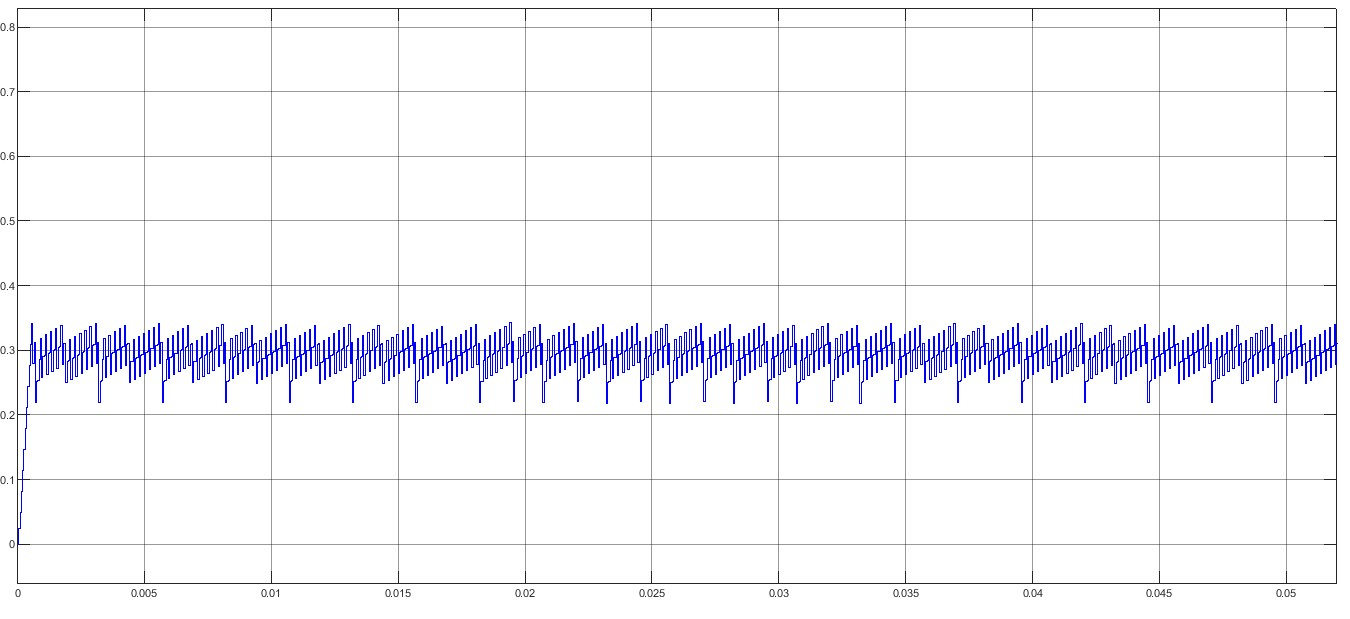
\includegraphics[width=0.8\textwidth]{Figures/charge.jpg} 
    \caption{Two Quadrant chopper inductor current profile during ESS Charging (Buck Mode).}
    \label{fig:current_response_buck}
\end{figure}

Assuming the PV panels operate at a peak power output of $5\text{ W}$, the current supplied to the DC link from the PV system is calculated as:
\begin{equation}
    I_{pvlink} = \frac{P_{PV}}{V_{dclink}} = \frac{5\text{ W}}{10\text{ V}} = 0.5\text{ A}
\end{equation}

Given that the EV battery load requires a constant charging current $I_{bucklink}$ of $0.2\text{ A}$, the dynamic reference current $I_{ref}$ directed to the storage system is computed via Kirchhoff's Current Law (KCL):
\begin{equation}
    I_{ref} = I_{pvlink} - I_{bucklink} = 0.5\text{ A} - 0.2\text{ A} = 0.3\text{ A}
\end{equation}

The simulation response for the inductor current under this condition is displayed in Figure 5.3. The current successfully settles at the $+0.3\text{ A}$ steady-state target within less than $1\text{ ms}$, exhibiting tight, high-frequency tracking within the configured hysteresis bounds.

\paragraph{Case 2: ESS Discharging / Boost Mode Operational Response}
To simulate environmental degradation (e.g., sudden cloud cover), the PV output power is stepped down to $1\text{ W}$. The corresponding current contribution from the solar interface drops to:
\begin{equation}
    I_{pvlink} = \frac{P_{PV}}{V_{dclink}} = \frac{1\text{ W}}{10\text{ V}} = 0.1\text{ A}
\end{equation}

To preserve the invariant $0.2\text{ A}$ required by the EV vehicle, the reference current equation yields:
\begin{equation}
    I_{ref} = I_{pvlink} - I_{bucklink} = 0.1\text{ A} - 0.2\text{ A} = -0.1\text{ A}
\end{equation}

The negative algebraic sign indicates an instantaneous reversal of power flow. The resulting inductor current profile is shown in Figure 5.4.

\begin{figure}[H]
    \centering
    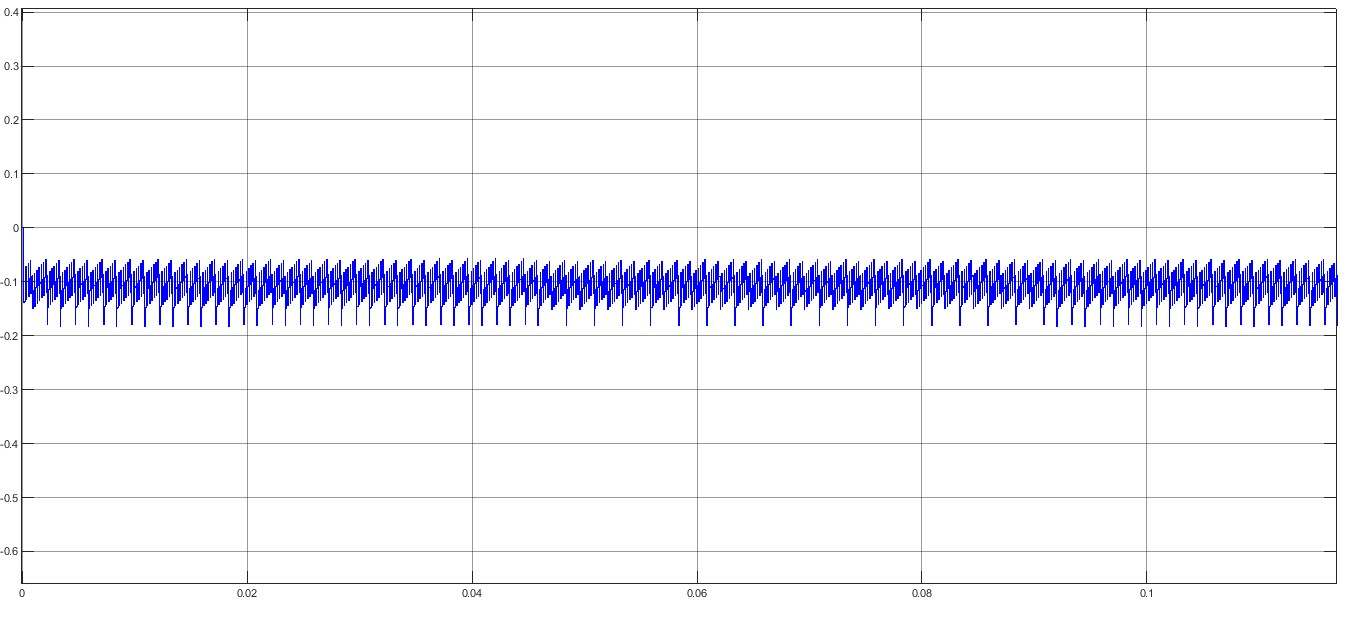
\includegraphics[width=0.8\textwidth]{Figures/discharge.jpg} 
    \caption{Two Quadrant chopper inductor current profile during ESS Discharging (Boost Mode).}
    \label{fig:current_response_boost}
\end{figure}

The system demonstrates excellent bidirectional agile tracking, stabilizing at $-0.1\text{ A}$ to inject power from the ESS back into the microgrid DC link, compensating for the solar deficit.

\paragraph{Switching Node Voltage Characteristics}
\begin{figure}[htbp]
    \centering
    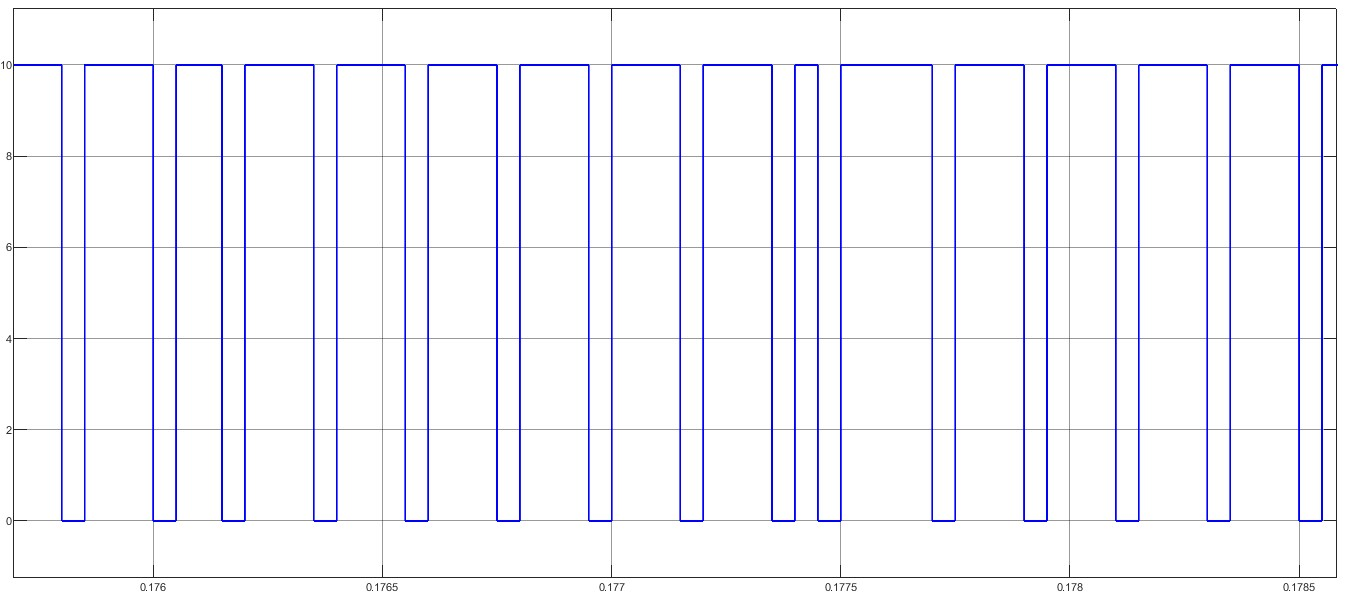
\includegraphics[width=0.8\textwidth]{Figures/vout.jpg} 
    \caption{Two Quadrant chopper switching node high-frequency voltage train.}
    \label{fig:switching_node_voltage_1}
\end{figure}

Figure 5.5 captures the high-frequency switching node voltage behavior of the chopper leg. The waveform shown is actually the Switching Node Voltage (or pole voltage) measured at the emitter of the top IGBT / collector of the bottom IGBT before the inductor stage.

As shown, the voltage pulses between $0\text{ V}$ (when $S_{bottom}$ is conducting or the low-side free-wheeling path is active) and $10\text{ V}$ (when $S_{top}$ is gated active). The variable-frequency characteristic visible in the pulse train is an inherent property of Hysteresis Current Control, which shifts its instantaneous switching frequency to maintain the current strictly within the designated error band regardless of transient state changes.

\subsubsection{Conclusion}
By establishing this bidirectional power flow framework, the 2Q Chopper effectively smooths out solar intermittency, guarantees a reliable charging routine for the electric vehicle, and enhances the overall self-sufficiency of the microgrid infrastructure. This section detailed the theoretical analysis, mathematical modeling, Simulink implementation, and closed-loop control strategies required to realize this robust 2Q Chopper energy management system.

% =========================================================================
% SUBSECTION 5.6.2: ADVANCED BIDIRECTIONAL CC-CV SUPERVISORY SYSTEM
% =========================================================================
\subsection{Advanced Bidirectional CC-CV Supervisory Energy Management System}

\subsubsection{Introduction}
To achieve true autonomy within a localized EV charging microgrid, the Two-Quadrant Chopper control loop must govern both active charging and active discharging cycles within rigorous electrochemical safety boundaries. While a standard current control loop handles short-term power fluctuations, it risks overcharging the ESS pack during sustained solar surpluses, or over-discharging (and destroying) the pack during sustained generation deficits.

While the baseline Hysteresis Current Control (HCC) manages fast power adjustments, a complete battery energy storage system (ESS) requires multi-stage boundaries to guarantee safety and longevity. Continuously charging at bulk current beyond the electrochemical saturation ceiling risks thermal stress, while deep-discharging below nominal cell chemistry limits can cause permanent capacity loss.
\newpage
To overcome these structural boundaries, a unified Bidirectional Constant Current / Constant Voltage (CC-CV) Energy Management Controller was developed. This supervisory system maintains active microgrid power stabilization under nominal states, but instantly transitions to voltage-clamping safety boundaries if the battery shifts toward a fully saturated or fully depleted state.

\subsubsection{Simulation Model}
\begin{figure}[H]
    \centering
    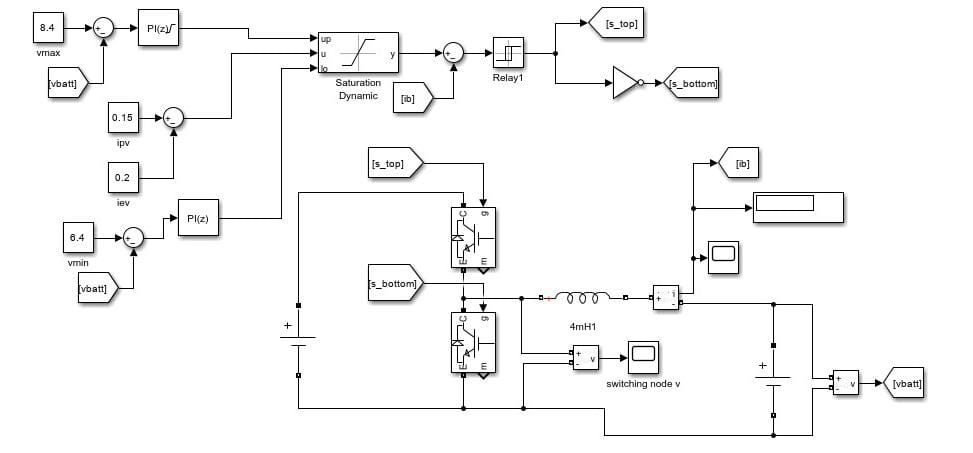
\includegraphics[width=0.8\textwidth]{Figures/CCCV.jpeg} 
    \caption{Two Quadrant chopper advanced closed-loop simulation model (CC-CV).}
    \label{fig:advanced_cccv_model}
\end{figure}

The complete architecture modeled within the MATLAB/Simulink environment is illustrated in Figure 5.6. The circuit consists of a high-voltage DC link representing the microgrid bus $V_{dclink} = 10\text{ V}$, a half-bridge IGBT/Diode switching leg, a power filtering inductor $L = 2\text{ mH}$, and a low-voltage battery storage system $V_{b} = 7.4\text{ V}$.

The supervisory logic uses a cascading control framework. The inner core relies on the high-bandwidth Hysteresis Current Modulator to manage immediate switching gate tracking. The outer supervisory envelope consists of two parallel Proportional-Integral (PI) voltage regulation loops feeding the control terminals of a dynamic Saturation block.

The net current demand derived from the photovoltaic microgrid balance is calculated continuously at the center summation node:
\begin{equation}
    I_{net} = I_{PV} - I_{EV}
\end{equation}

This reference signal is fed directly into a Saturation block whose upper limit $u_{limit}$ and lower limit $l_{limit}$ are dynamically governed by the safe operational voltage boundaries:

\vspace{1.5ex}
\noindent\textbf{Nominal CC Mode: }\\
While the battery terminal voltage $V_{batt}$ satisfies $6.4\text{ V} < V_{batt} < 8.4\text{ V}$, both outer loop PI controllers saturate at their maximum absolute operating limits. Consequently, the calculated microgrid current passes through the Saturation block unconstrained:
\begin{equation}
    I_{ref^*} = I_{net}
\end{equation}

\vspace{1.5ex}
\noindent\textbf{CV Charging Overvoltage Clamp:}\\
If $V_{batt}$ reaches the $8.4\text{ V}$ maximum safety limit $V_{max}$, the upper PI loop activates. It forces the upper limit $u_{limit}$ threshold down, restricting the reference current to follow an exponential decay profile:
\begin{equation}
    u_{limit} = K_{p1} \cdot (V_{max} - V_{batt}) + K_{i1} \cdot \int (V_{max} - V_{batt}) \cdot dt
\end{equation}

\vspace{1.5ex}
\noindent\textbf{CV Discharging Cutoff Clamp:}\\
If $V_{batt}$ drops to the $6.4\text{ V}$ deep discharge floor $V_{min}$, the lower PI loop assumes control. It restricts the lower limit $l_{limit}$ to clip negative current injection, maintaining cell equilibrium:
\begin{equation}
    l_{limit} = K_{p2} \cdot (V_{min} - V_{batt}) + K_{i2} \cdot \int (V_{min} - V_{batt}) \cdot dt
\end{equation}

\subsubsection{Principle of Operation}
To understand how this advanced control architecture works, we must trace the loop signals from left to right. This simulation uses the Saturation Block as a dynamic ``traffic controller'' or decision-maker that automatically switches between Constant Current (CC) and Constant Voltage (CV) modes depending on physical system states.

\paragraph{Stage 1: The Net Current Reference (The Middle Path)}
\begin{equation}
   I_{net} = I_{PV} - I_{EV}
\end{equation}
This $I_{net}$ represents the exact net current your battery wants to supply to the ESS (since PV panels produced excess power) or to discharge to support the EV charging load (since the PV panels are falling short). This signal enters the middle port ($u$) of the Saturation Block. Under normal operating conditions, if the battery voltage is safe, this block acts like a clear window: whatever enters port ($u$) passes straight through to the output $y$.

\paragraph{Stage 2: The Dynamic Guardrails (The PI Control Loops)}
This is where the advanced supervisory control layer takes over. Instead of using fixed constant numerical boundaries for the upper and lower limits of the Saturation block, the thresholds are fed with variable, real-time tracking signals coming from the parallel PI controllers.

\begin{enumerate}
    \item \textbf{The Upper Guardrail (Overvoltage Protection):} 
    \begin{itemize}
        \item \textbf{Target Reference Parameter:} $V_{max} = 8.4\text{ V}$.
        \item \textbf{Input Error Loop:} The block compares $V_{max}$ directly with the actual feedback battery voltage $V_{batt}$.
        \item \textbf{Behavior:} As long as $V_{batt}$ remains safely below $8.4\text{ V}$ (e.g., at $7.4\text{ V}$), the calculated error is large and positive. The PI controller responds by outputting its maximum design limit, forcing the upper boundary ($up$) of the Saturation block to stay wide open.
        \item \textbf{The Switchover Handoff:} If the battery charges up and $V_{batt}$ intersects the $8.4\text{ V}$ ceiling, the tracking error drops to zero. The PI controller instantly wakes up, exits saturation, and lowers its output. It shrinks the upper limit ($up$) of the Saturation block, squeezing the current down toward $0\text{ A}$ to lock the battery voltage at exactly $8.4\text{ V}$ (\textit{CV Charging Mode}).
    \end{itemize}
    
    \item \textbf{The Lower Guardrail (Undervoltage Protection):}
    \begin{itemize}
        \item \textbf{Target Reference Parameter:} $V_{min} = 6.4\text{ V}$.
        \item \textbf{Input Error Loop:} The block compares $V_{min}$ directly with the actual feedback battery voltage $V_{batt}$.
        \item \textbf{Behavior:} While the battery terminal voltage $V_{batt}$ remains safely above the critical low-voltage floor $V_{min} = 6.4\text{ V}$, the error signal fed into the lower PI controller is negative ($V_{min} - V_{batt} < 0$). This forces the PI regulator to saturate at its maximum lower design limit. Because this lower clamp threshold $l_{limit}$ is set much deeper than the required discharge current, the Saturation block does not clip the signal. The net current reference passes through to the inner hysteresis loop completely unconstrained, maintaining standard \textit{Constant Current (CC) Discharging Mode}.
        \item \textbf{The Switchover Handoff:} If $V_{batt}$ drops all the way down to the critical $6.4\text{ V}$ floor, the lower PI controller stops saturating. It actively increases its output, clamping the lower limit ($lo$) of the Saturation block. This forces the negative discharging current back up toward $0\text{ A}$, clamping the battery at $6.4\text{ V}$ and preventing deep-discharge cell failure (\textit{CV Discharging Mode}).
    \end{itemize}
\end{enumerate}

\paragraph{Stage 3: The Hysteresis Engine}
Once the Saturation block decides on the final, safe current reference $I_{ref^*}$, it passes it directly to the subtraction block right before the relay stage:
\begin{equation}
   e(t) = I_{ref^*} - I_{b}
\end{equation}

This tracking error $e(t)$ is fed into the Hysteresis Relay Block. The relay does not use PWM carriers; instead, it utilizes a standard bang-bang switching strategy:
\begin{itemize}
    \item \textbf{When current is too low} ($e(t) > +\text{band}$): The relay outputs a logical 1. This fires a signal to $S_{top}$, turning the upper IGBT ON and the lower IGBT OFF via a hardware NOT gate inverter. Current starts ramping up through the filtering inductor from the $10\text{ V}$ DC link.
    \item \textbf{When current is too high} ($e(t) < -\text{band}$): The relay switches to a logical 0. $S_{top}$ shuts off, and the inverter forces $S_{bottom}$ ON. The switching node side of the inductor is pulled down to $0\text{ V}$ ground, causing the inductor current to ramp back down.
\end{itemize}
By bouncing back and forth between these two limits instantly, the closed hysteresis loop keeps the battery current locked firmly onto the reference target.

\subsubsection{Simulation Results and Discussion}

\paragraph{Case 1: ESS Charging / Buck Mode Control Profiles}
Assuming the PV panels operate at a peak power output of $5\text{ W}$, the current supplied to the DC link from the PV system is calculated as:
\begin{equation}
    I_{pv} = \frac{P_{PV}}{V_{dclink}} = \frac{5\text{ W}}{10\text{ V}} = 0.5\text{ A}
\end{equation}

Given that the EV battery load requires a constant charging current $I_{ev}$ of $0.2\text{ A}$, the dynamic reference current $I_{ref}$ directed to the storage system is computed via KCL:
\begin{equation}
    I_{ref} = I_{pv} - I_{ev} = 0.5\text{ A} - 0.2\text{ A} = 0.3\text{ A}
\end{equation}

When $V_{batt} = 7.4\text{ V}$, constant current charging takes place smoothly at a charging current target of $+0.3\text{ A}$ as verified by the profile in Figure 5.7.

\begin{figure}[H]
    \centering
    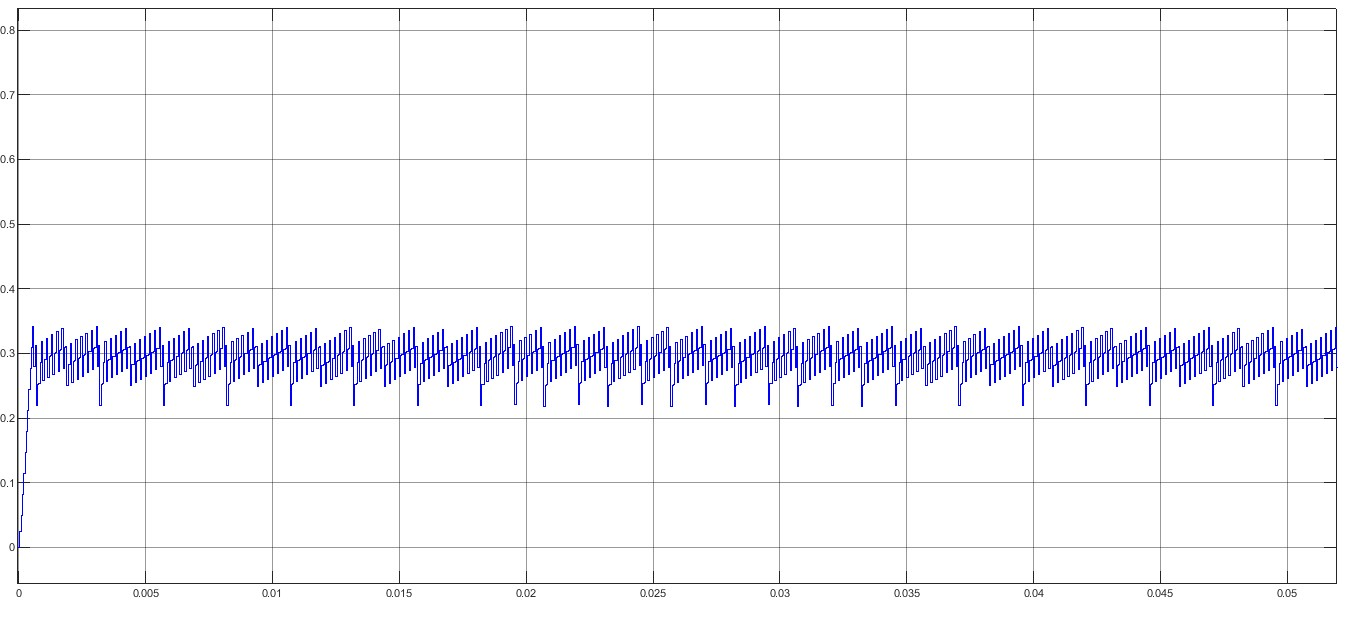
\includegraphics[width=0.8\textwidth]{Figures/7.4CC.jpg} 
    \caption{Two Quadrant chopper inductor current under CC charging control loop ($V_{batt} = 7.4\text{ V}$).}
    \label{fig:current_cc_charging_74}
\end{figure}

When the state variable tracks up to $V_{batt} = 8.4\text{ V}$, the loop automatically triggers the switchover execution to constant voltage control mode, forcing the current profile down to a zero steady-state line to avoid cellular overcharging, as illustrated in Figure 5.8.

\begin{figure}[H]
    \centering
    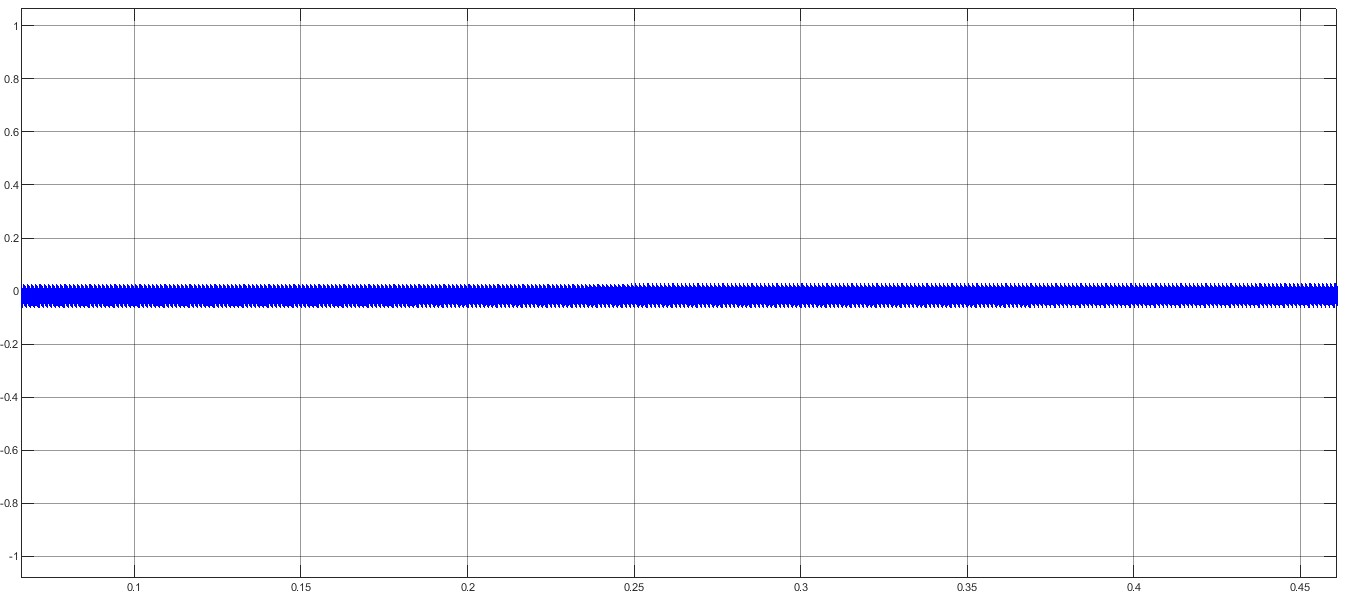
\includegraphics[width=0.8\textwidth]{Figures/8.4CV.jpg} 
    \caption{Two Quadrant chopper inductor current profile decaying to zero under CV charging protection clamp ($V_{batt} = 8.4\text{ V}$).}
    \label{fig:current_cv_charging_84}
\end{figure}

\paragraph{Case 2: ESS Discharging / Boost Mode Control Profiles}
To simulate environmental degradation (e.g., sudden cloud cover), the PV output power is stepped down to $1\text{ W}$. The corresponding current contribution from the solar interface drops to:
\begin{equation}
    I_{pv} = \frac{P_{PV}}{V_{dclink}} = \frac{1\text{ W}}{10\text{ V}} = 0.1\text{ A}
\end{equation}

To preserve the invariant $0.2\text{ A}$ required by the EV vehicle, the reference current equation yields a negative target:
\begin{equation}
    I_{ref} = I_{pv} - I_{ev} = 0.1\text{ A} - 0.2\text{ A} = -0.1\text{ A}
\end{equation}

When $V_{batt} = 7.4\text{ V}$, constant current discharging takes place at a regulated current line of $-0.1\text{ A}$ as shown in Figure 5.9.

\begin{figure}[H]
    \centering
    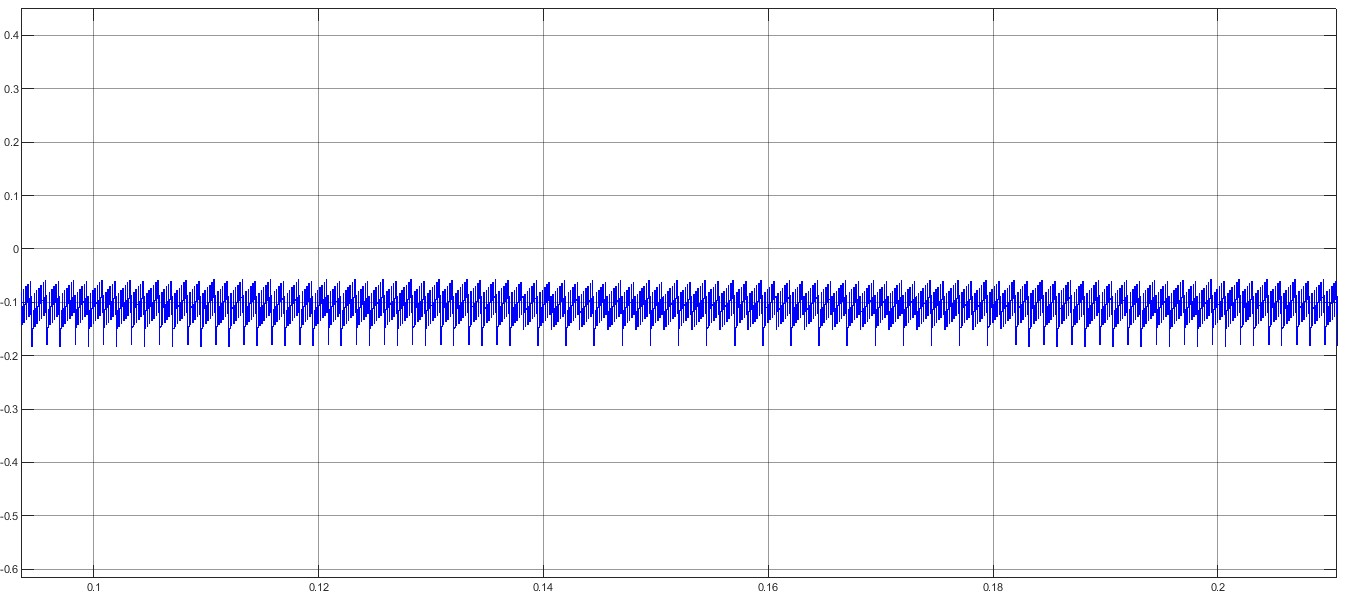
\includegraphics[width=0.8\textwidth]{Figures/7.4 DISCC.jpg} 
    \caption{Two Quadrant chopper inductor current under CC discharging control loop ($V_{batt} = 7.4\text{ V}$).}
    \label{fig:current_cc_discharging_74}
\end{figure}

When the cell drains down to the critical low-voltage floor threshold $V_{batt} = 6.4\text{ V}$, the controller switches execution layers to constant voltage control, clipping the negative discharging current back to $0\text{ A}$ to isolate the battery from deep-discharge cell failure, as shown in Figure 5.10.

\begin{figure}[H]
    \centering
    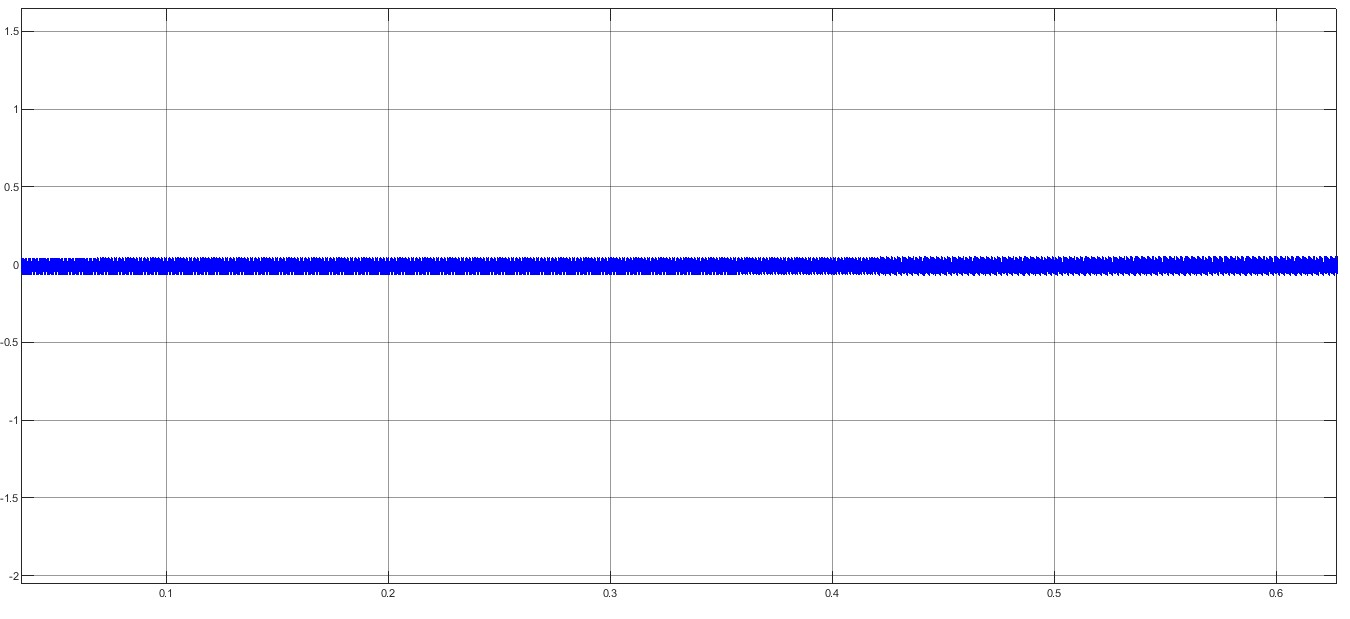
\includegraphics[width=0.8\textwidth]{Figures/6.4 CVDIS.jpg} 
    \caption{Two Quadrant chopper inductor current under CV discharging cutoff clamp protection ($V_{batt} = 6.4\text{ V}$).}
    \label{fig:current_cv_discharging_64}
\end{figure}

\paragraph{Switching Node Voltage Characteristics}
The high-frequency switching pulse train behavior measured across the synchronous branch under CC-CV mode is captured within the graph in Figure 5.11.

\begin{figure}[H]
    \centering
    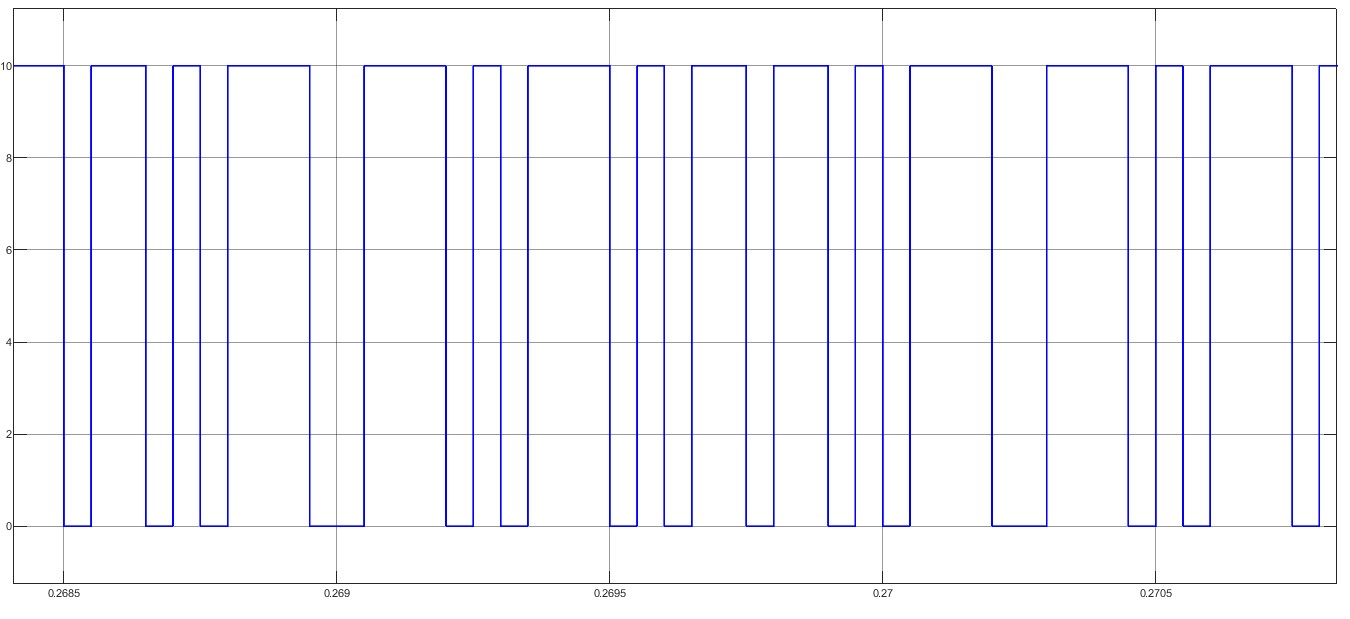
\includegraphics[width=0.8\textwidth]{Figures/switchingnodev.jpg} 
    \caption{Advanced CC-CV chopper switching node high-frequency voltage train.}
    \label{fig:switching_node_voltage_2}
\end{figure}

\subsubsection{Conclusion}
The dynamic responses captured across the simulation timelines verify the operation of the control logic. As shown in the steady-state measurements, the inductor current cleanly tracks the reference target, settling closely near the nominal target within a localized hysteresis ripple band.

When the threshold limit boundaries are intersected, the cascading PI loops smoothly restrict the saturation limits. This changes the reference envelope seamlessly, eliminating high-frequency oscillations or current transient overshoots at the handoff point. This confirms the robustness of the combined control design under both step changes and continuous charging profiles.